%% Parler de data.ina.fr : parce que nous aussi on permet d'avoir plusieurs clefs d'entrée etc... A la conclusion de toute fin dire que la réalisation du projet est incertain et dépend de l'aboutissement d'autres projet (comme Notilus et compagnie)
\subsection{La découvrabilité dans les institutions patrimoniales}

%% Introduction : Définition de la découvrabilité %%

La \enquote{découvrabilité}, dans l'environnement numérique, se définit comme la capacité à voir, accéder et consulter un contenu parmi un ensemble important d'autres contenus\footcite{decouvrabilite}. On le différencie de la repérabilité, qui définit la capacité à trouver un contenu en ligne, par son caractère non intentionnel. Un contenu est découvrable si un utilisateur peut s'y trouver confronté, sans que cela soit son intention première. Au cours des dernières années, cette notion a pris une grande importance pour les institutions patrimoniales, notamment lors du basculement de la consommation des contenus en ligne avec le confinement\footcite{decouvrabilite}. Cette notion s'applique en général au contenu sur le web mais ce n'est pas le cas dans ce projet. Précédemment, nous avons constaté que, grâce au web et aux réseaux sociaux, l'INA est aujourd'hui une institution de référence en matière d'archives audiovisuelles. Il est fort probable qu'une personne francophone, à la recherche de contenus audiovisuels d'archives finira par entrer en contact avec un site ou un réseau social de l'INA. Nous en avons nous-même fait l'expérience en tentant de nous mettre dans la peau de ce profil. Dans le contexte d'une recherche en ligne avec le moteur de recherche Google, le site de l'INA \enquote{ina.fr} est le premier résultat aux recherches \enquote{vidéos d'archives}, \enquote{archives audiovisuelles} et il apparaît dans la première page de résultat avec les recherches \enquote{Cinq colonnes à la une}, \enquote{anciennes émissions tv}, \enquote{début TF1}, \enquote{passage à la couleur tv france}. Dans le contexte des réseaux sociaux, il est plus difficile de déterminer la vitesse à laquelle nous pouvons rencontrer un contenu de l'INA ou de toute autre institution patrimoniale car le fonctionnement algorithmique des réseaux sociaux est très opaque et change régulièrement\footcite[252]{farchy2023}. Nous pouvons tout de même supposer que la production de parodies de documents diffusés par l'INA ou la production de fausses archives par intelligence artificielle génératives reproduisant les codes de ce même document sont tous deux des indicatifs de la forte présence de l'INA sur le web et les réseaux sociaux. 

Nous avons pu constater, au cours du développement de cet exposé, que la découvrabilité des contenus des institutions patrimoniales est une problématique au centre des stratégies de communications de ces institutions, y compris l'INA. C'est pourquoi l'outil que nous souhaitons mettre en place n'a pas pour objectif d'améliorer la découvrabilité des collections de l'INA sur le web mais plutôt la découvrabilité de tous ses documents dans ses bases de données. Actuellement, la principale méthode d'utilisation des bases de données de l'INA est de savoir ce que l'on recherche tout en possédant une connaissance des changements de politiques documentaires s'appliquant aux périodes qui nous intéressent. La découvrabilité est restreinte car l'outil de consultation Hyperbase n'a pas été pensé dans un objectif de découvrabilité mais de recherche.

\subsection{Cartographier les données}
%% Définition de datavisualisation %%

Le premier outil auquel nous avons eu recours pour faciliter l'accessibilité aux collections est la datavisualisation. Elle permet de mobiliser une quantité massive de données afin d'en faire ressortir des informations plus accessibles à l'échelle de l'utilisateur. Grâce à cet outil, il est possible de faire correspondre une quantité importante de données à des structures graphiques\footcite[][42]{fourlinnie2016} permettant à un utilisateur ne connaissant pas ces bases de données de comprendre ce qu'elles contiennent et ce qu'il peut y trouver. Face aux données massives que représentent les collections numériques de l'INA, c'est un outil qui est précieux. Par l'utilisation de formes graphiques, nous pouvons simplifier la complexité des bases de données de l'institut. 

%% Premier type d'utilisation : Vision globale des données de toute la collection %%

Parmi les différentes manières de représenter nos données, la première, et celle qui semble la plus évidente, est de réaliser une visualisation de l'ensemble des collections. C'est ce qu'a fait le laboratoire de recherche de la bibliothèque publique de New-York (NYPL Labs) en réalisant une projection graphique de leurs collections. Ils ont rapproché les différents sujets indexés dans leur collections selon le nombre d’occurrence de ceux-ci dans les ouvrages de leurs collections. Plus un terme d'indexation apparaît, plus la \enquote{bulle} qui lui associée est grosse.

\begin{figure}[H]
	\centering
	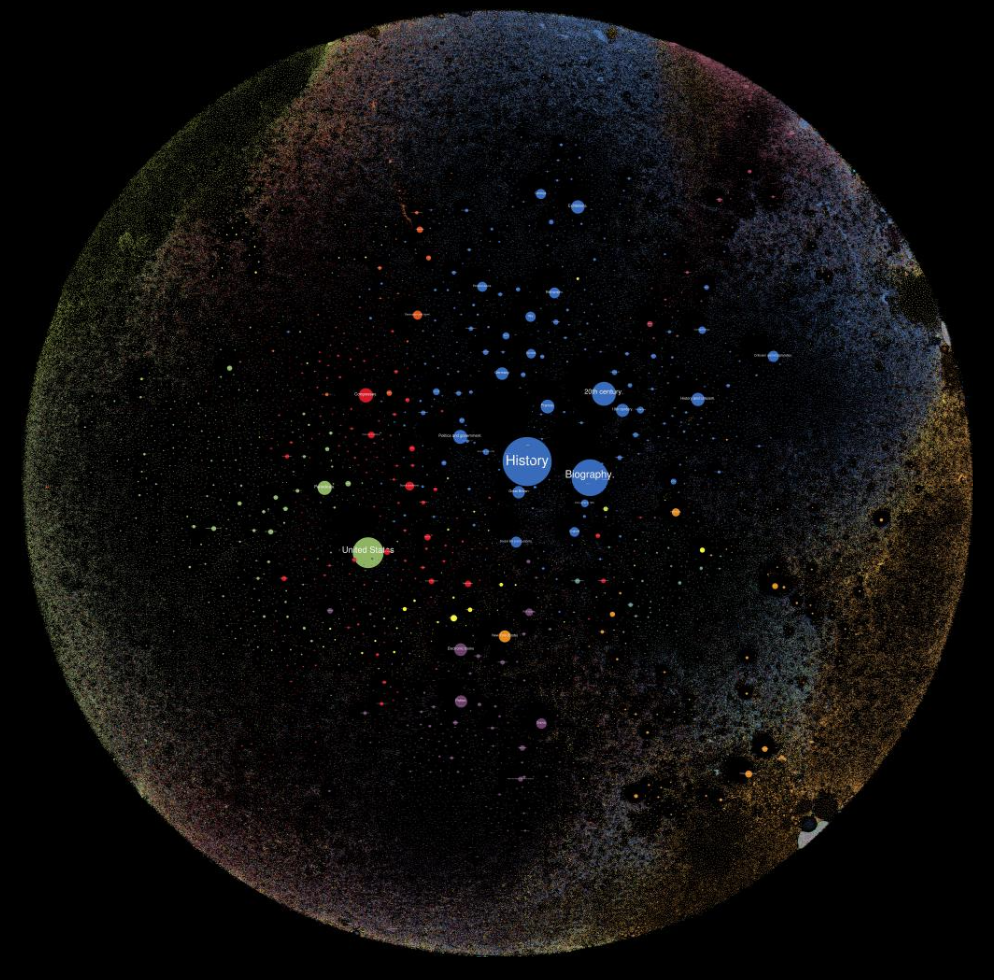
\includegraphics[width=0.70\linewidth]{./illustrations/NYPL_graph.png}
	\caption{Capture d'écran du graphique de la NYPL Lab}
	\label{fig:NYPL_graph}
\end{figure}

%% Application à l'INA %%

Cet exemple nous permet de questionner les données à choisir lors de la conception d'une visualisation de données : quelles informations à quels questions cette visualisation doit-elle répondre ? Selon l'angle que nous abordons dans ce mémoire, il n'est pas pertinent de faire ressortir les données d'indexation des collections comme l'exemple cité précédemment car notre outil est concentré sur la compréhension du traitement documentaire des collections. Faire ressortir les données d'indexation ne ferait qu'accentuer le manque de visibilité des collections n'étant pas indexées. Pire, car nous pouvons toujours utiliser cette visualisation pour mettre en avant les documents non indexés, ce qui en un sens illustrerait une histoire de l'institution que nous avons déjà précédemment décrit. Mais quid des documents indexés avec des termes désuets qui disparaîtraient totalement dans la masse, ce qui irait à l'encontre de cette volonté d'utiliser les datavisualisations pour accompagner l'utilisateur dans l'exploration de ces collections avec un traitement documentaire inégal. Notre objectif est de faire ressortir la richesse de notre base de données, pas d'accentuer ses défauts. Dans le cadre de l'utilisation de datavisualisations au service de la découvrabilité des collections, nous souhaitons utiliser ce premier type de datavisualisations afin d'introduire l'utilisateur aux différences de traitement documentaire qui se présenterons lors de son exploration de la base de données. C'est pourquoi, nous avons fait le choix de présenter aux utilisateurs, sur la première page de notre outil, une visualisation en bulles groupées de l'ensemble des collections\footnote{Toutes les visualisations de données ont été réalisées sur Tableau Public avec une extraction de la base de données du dépôt légal DLTV contenant toutes les émissions en première diffusion de la chaîne France 2 et Arte, voir Annexe \ref{ann:cdc},\nameref{ann:cdc}), p.~\pageref{ann:cdc}.}. 

\begin{figure}[H]
	\centering
	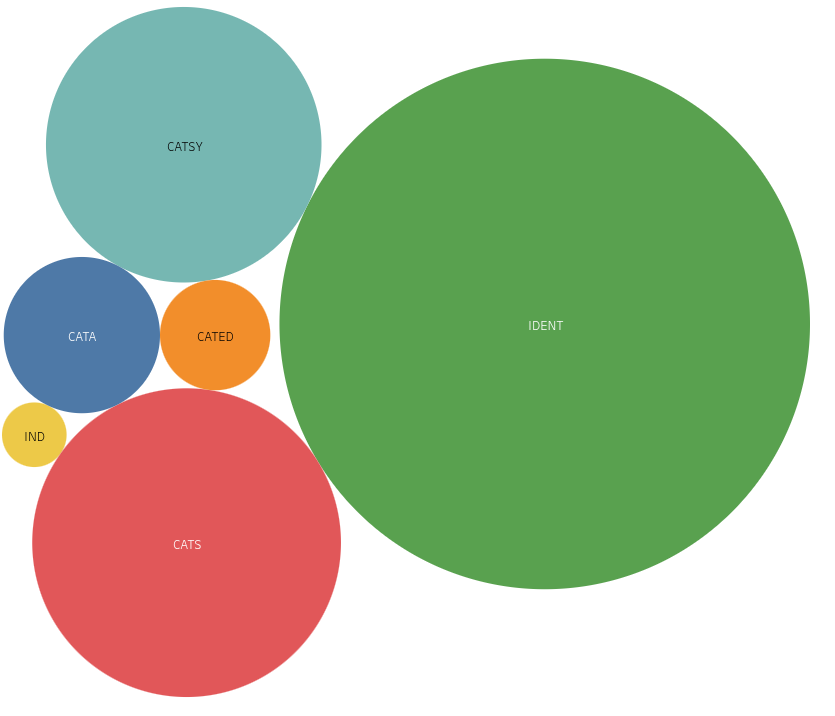
\includegraphics[width=0.75\linewidth]{./illustrations/graph_ina_tout.png}
	\caption{Graphique en bulles groupées du traitement documentaire dans les bases de données de l'INA}
	\label{fig:graph_ina1}
\end{figure}

Ce graphique permet à l'utilisateur de faire une première entrée dans la base de données et d'en comprendre la composition. Il a la double fonction d'introduire l'utilisateur aux informations qu'il peut trouver dans la base de données et de servir d'illustration à un texte expliquant les différents traitements appliqués aux documents, dans une version bien plus simplifiée, semblable aux connaissances que dispenseraient les documentalistes de l'INAthèque. Cela dit, grâce à cette visualisation, l'utilisateur comprend que les données qu'il va exploiter n'ont pas un traitement égal, mais cela ne suffit pas à permettre la découverte des collections. Tout au long de ce mémoire, nous avons à de multiples reprises appuyé sur le fait que ce manque d'accessibilité aux données étaient dues à un enchaînement de politique documentaire. En conséquent, il est important de prendre en considération les données temporelles dans nos datavisualisations. 

%% Image d'un phénomène non perceptible visuellement %%

Pour cela, une vue chronologiques des données permet de démontrer l'évolution de ces pratiques documentaires. C'est l'idée qui est mise en avant par la représentation chronologique de l'entrée des données des arbres et plantes conservées dans l'aboretum de Harvard\footcite{loukissas}. Cette base de données est également marquée par des changements de politiques documentaires, dans ce cas ce sont les numéros d'accessions dont la logique d'élaboration a été affectée par différentes politiques documentaires. Cette visualisation permet de mettre en avant l'activité d'indexation dans le temps.

%% Application à l'INA %% 

Cette visualisation est plus pertinente dans notre démarche de médiation du traitement documentaire de collections patrimoniales. Elle permet à l'utilisateur de ces bases de données de comprendre en un coup d’œil la situation des collections qu'il consulte et aviser ses pratiques en conséquence. Il peut se diriger vers le traitement qui contiendra les données qu'il recherche ou adapter sa recherche aux champs que comprennent les notices qu'il désire. En adoptant une approche temporelle, cette visualisation est particulièrement adaptée à une étude historiques. La visualisation qui suit a été crée avec l'outil \enquote{Tableau Public}, d'après une extraction de toutes les notices d'émissions en première diffusion de la chaîne France 2 sur la base de données du dépôt légal.

\begin{figure}[H]
	\centering
	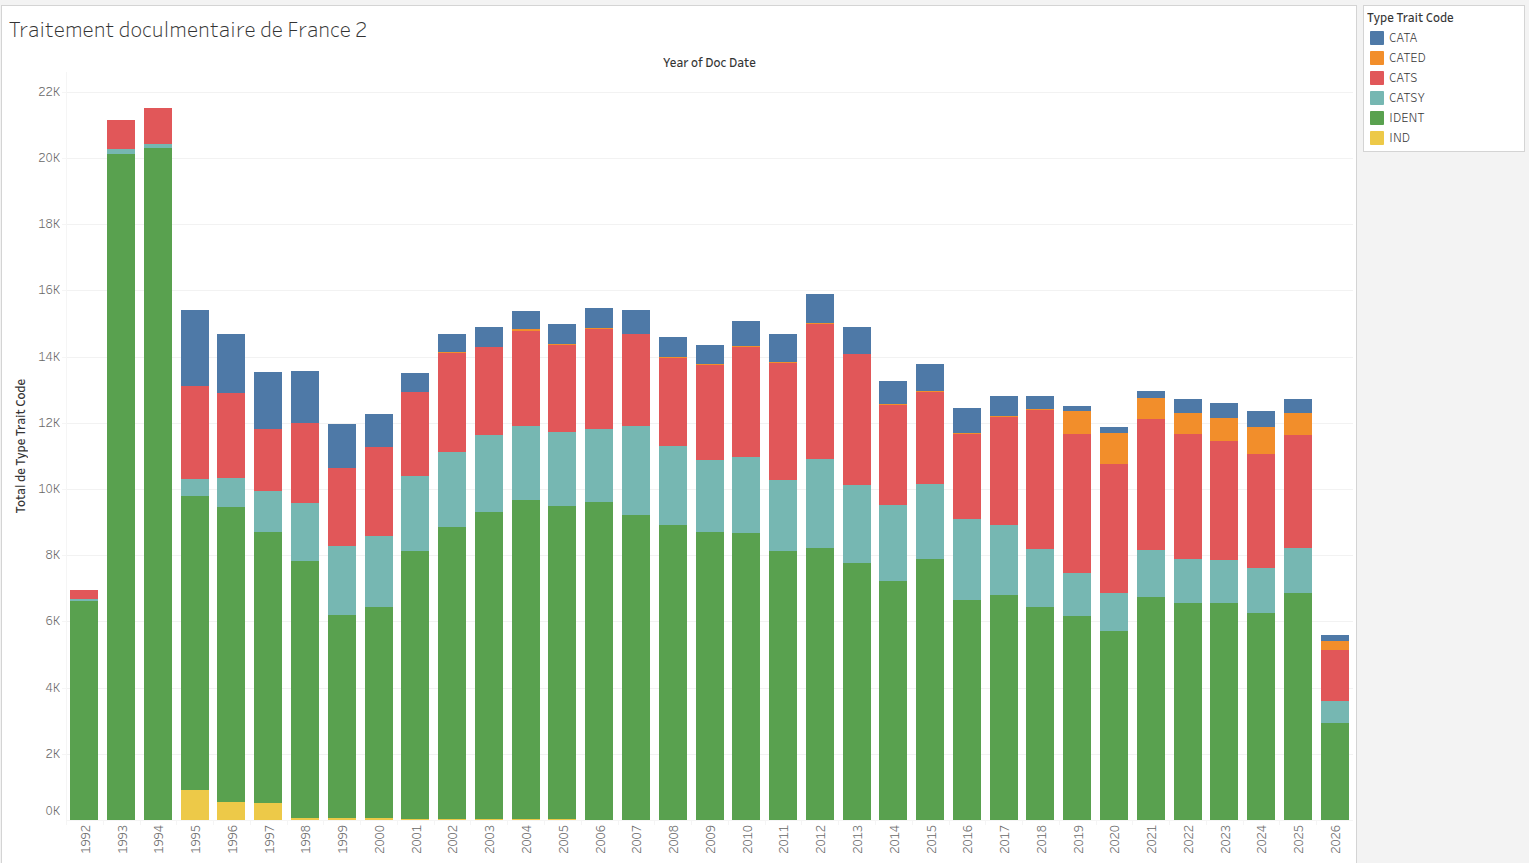
\includegraphics[width=1\linewidth]{./illustrations/traitement_FR2.png}
	\caption{Visualisation du traitement documentaire chronologique de la chaine \enquote{France 2}}
	\label{fig:traitement_FR2}
\end{figure}

Dans ce graphique en barre réalisé sur les données de la chaîne télévisée France 2, l'utilisateur peut récupérer en quelques instants les informations dont il peut avoir besoin. Sur l'axe des ordonnées s'affiche le nombre de notices et sur l'axe des abscisses les années. Grâce à ce graphique, l'utilisateur peut donc savoir le nombre d'émissions traitées chaque année ainsi que le traitement le plus utilisé, à la fois pour chaque année mais aussi sur l'ensemble de la période durant laquelle cette chaîne a été traité. Grâce à ces informations, tirées des données des bases de l'INA et mis en forme grâce à ce graphique l'utilisateur a une vue générale sur le traitement documentaire de cette chaîne et peut donc orienter ses recherches sur la période durant lesquelles le traitement correspond aux informations qu'il recherche ou au contraire, si il a déjà effectué une recherche sur cette chaîne, sans succès, il peut comprendre pourquoi. Le présent exemple fonctionne sur une chaîne mais également sur un programme isolé ou même sur un genre.

\begin{figure}[H]
	\centering
	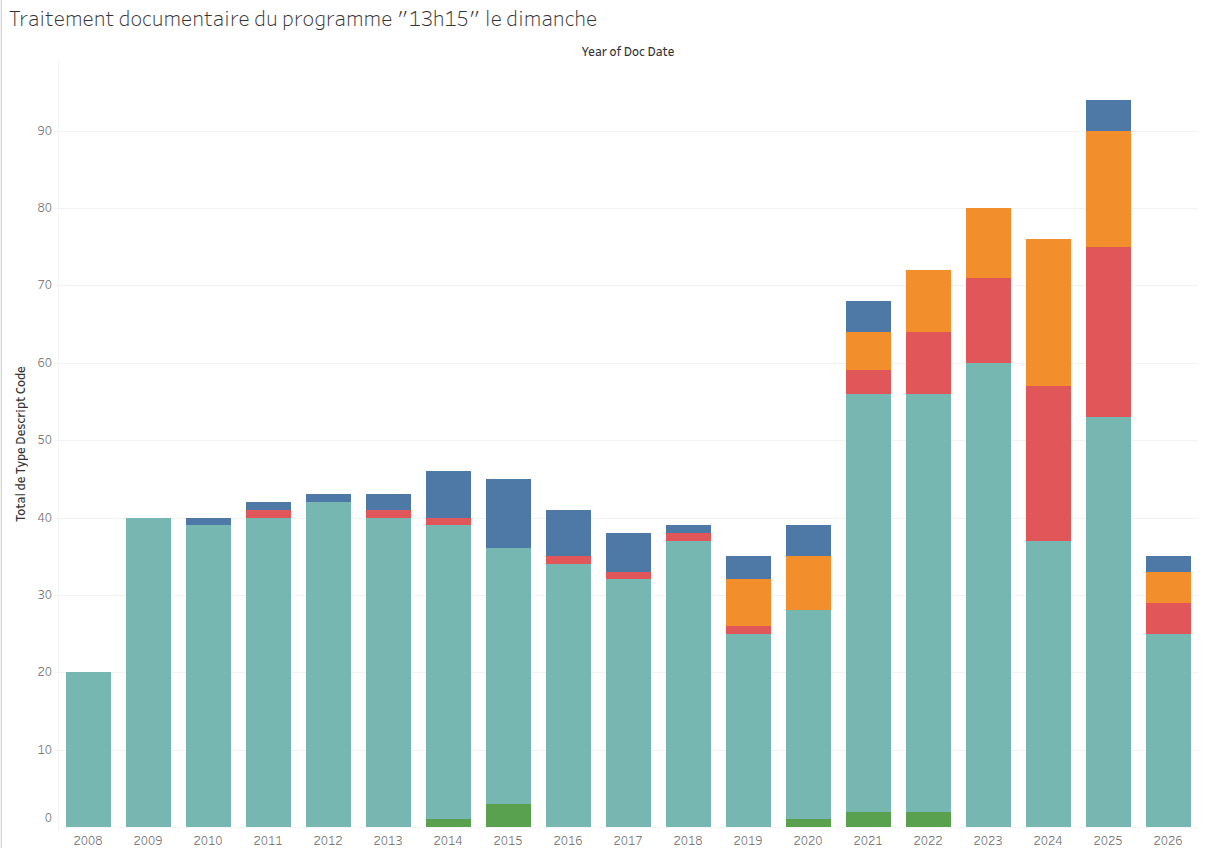
\includegraphics[width=0.75\linewidth]{./illustrations/graph_ina_programme.png}
	\caption{Visualisation du traitement documentaire chronologique du programme \enquote{13h15 le dimanche}}
	\label{fig:traitement_13h15}
\end{figure}

\begin{figure}[H]
	\centering
	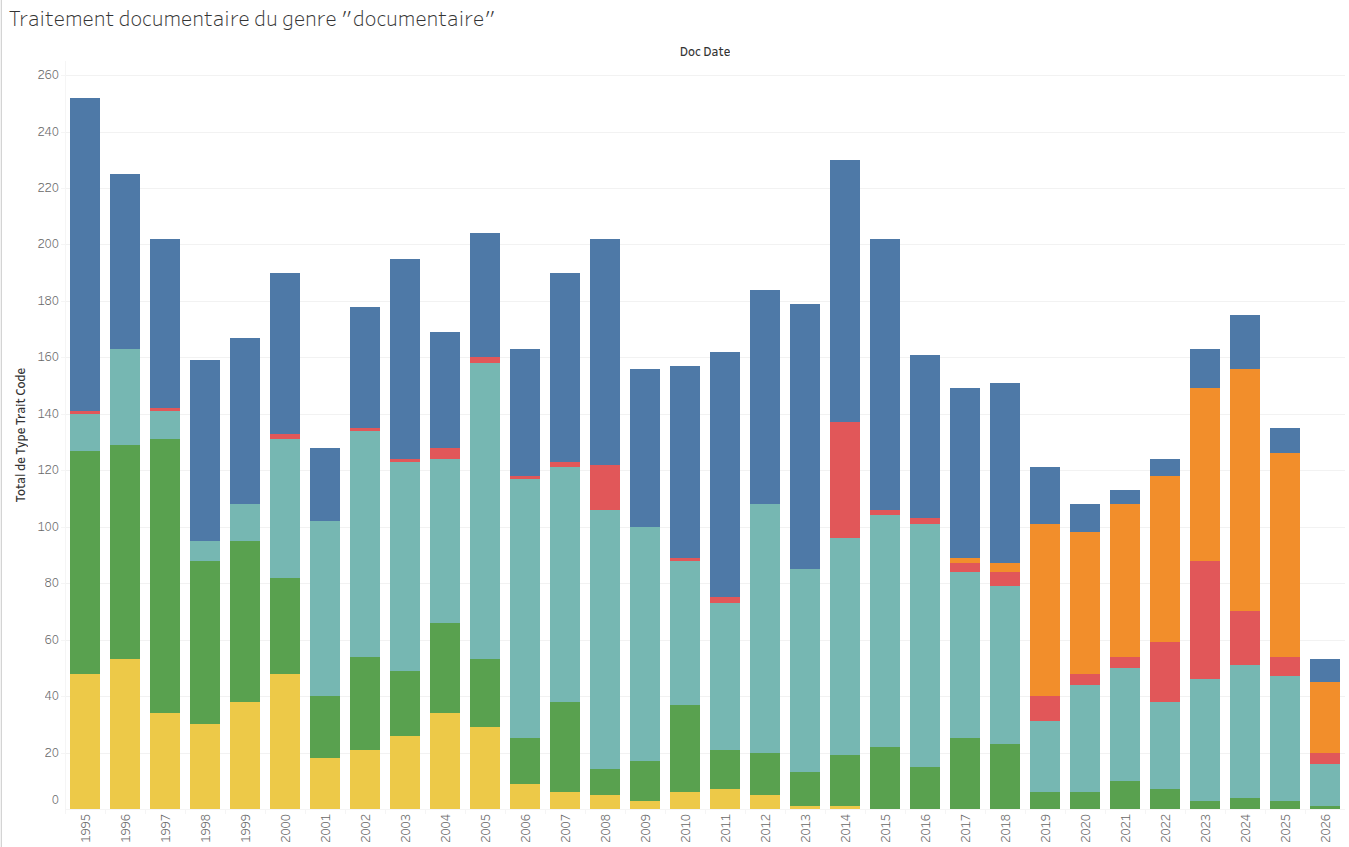
\includegraphics[width=0.75\linewidth]{./illustrations/graph_ina_genre.png}
	\caption{Visualisation du traitement documentaire chronologique du genre \enquote{documentaire}}
		\label{fig:traitement_docu}
	\end{figure}
	
En mettant à disposition toutes ces datavisualisation, mettant à contribution les données des dates de diffusions et du type de traitement appliqué, nous parvenons à donner aux utilisateurs trois différentes portes d'entrée dans les données. 

%% Utilisation de l'INA pour la découvrabilité : data.ina.fr : Montrer que c'est courant d'utiliser les datavisualisations pour améliorer la découvrabilité des données %%